\documentclass[]{article}

% Imported Packages
%------------------------------------------------------------------------------
\usepackage{amssymb}
\usepackage{amstext}
\usepackage{amsthm}
\usepackage{amsmath}
\usepackage{enumerate}
\usepackage{fancyhdr}
\usepackage[margin=1in]{geometry}
\usepackage{graphicx}
%\usepackage{extarrows}
%\usepackage{setspace}
%\usepackage{xcolor}
\usepackage{color}
\graphicspath{ {./images/} }
%------------------------------------------------------------------------------

% Header and Footer
%------------------------------------------------------------------------------
\pagestyle{plain}  
\renewcommand\headrulewidth{0.4pt}                                      
\renewcommand\footrulewidth{0.4pt}                                    
%------------------------------------------------------------------------------

% Title Details
%------------------------------------------------------------------------------
\title{Deliverable \#1 Template : Software Requirement Specification (SRS)}
\author{SE 3A04: Software Design II -- Large System Design}
\date{}
                            
%------------------------------------------------------------------------------

% Document
%------------------------------------------------------------------------------
\begin{document}

\maketitle
\noindent{\bf Tutorial Number:} T03\\
{\bf Group Number:} G06 \\
{\bf Group Members:}
\begin{itemize}
	\item Virochaan Ravichandran Gowri
	\item Alex Yoon
	\item Noah Goldschmied
	\item Krish Dogra
	\item Leo Vugert
\end{itemize}

\section*{IMPORTANT NOTES}
\begin{itemize}
	\item Be sure to include all sections of the template in your document regardless whether you have something to write for each or not
	      \begin{itemize}
		      \item If you do not have anything to write in a section, indicate this by the \emph{N/A}, \emph{void}, \emph{none}, etc.
	      \end{itemize}
	\item Uniquely number each of your requirements for easy identification and cross-referencing
	\item Highlight terms that are defined in Section~1.3 (\textbf{Definitions, Acronyms, and Abbreviations}) with \textbf{bold}, \emph{italic} or \underline{underline}
	\item For Deliverable 1, please highlight, in some fashion, all (you may have more than one) creative and innovative features. Your creative and innovative features will generally be described in Section~2.2 (\textbf{Product Functions}), but it will depend on the type of creative or innovative features you are including.
\end{itemize}

\newpage
\section{Introduction}
\label{sec:introduction}
% Begin Section

\begin{itemize}
	\item Provide an overview of the document/SRS.
\end{itemize}


\subsection{Purpose}
\label{sub:purpose}
% Begin SubSection
This Software Requirement Specification has been created to specify the requirements needed to develop a secure communication app (VanklComm) for our organization. This SRS will ensure to cover functional requirements specifying how the app will perform the secure communication, including viewpoints from stakeholders and common business events and use cases and non-functional requirements outlining specifications of the system.
% End SubSection

\subsection{Scope}
\label{sub:scope}
% Begin SubSection
\begin{itemize}
	\item Identify the software product(s) to be produced, and name each (e.g., Host DBMS, Report Generator, etc.)
	\item Explain what the software product(s) will do (and, if necessary, also state what they will not do).
	\item Describe the application of the software being specified, including relevant benefits, objectives, and goals.
	      %	\item Be consistent with similar statements in higher-level specifications (e.g., the system requirements specification), if they exist
\end{itemize}
% End SubSection

\subsection{Definitions, Acronyms, and Abbreviations}
\label{sub:definitions_acronyms_and_abbreviations}
% Begin SubSection
\begin{itemize}
	\item Provide the definitions of all terms, acronyms, and abbreviations required to properly interpret the SRS.
	\item This should be in alphabetical order.
\end{itemize}
% End SubSection

\subsection{References}
\label{sub:references}
% Begin SubSection
\begin{itemize}
	\item Provide a complete list of all documents referenced elsewhere in the SRS.
	\item Identify each document by title, report number (if applicable), date, and publishing organization.
	\item Specify the sources from which the references can be obtained.
	\item Order this list in some sensible manner (alphabetical by author, or something else that makes more sense).
\end{itemize}
% End SubSection

\subsection{Overview}
\label{sub:overview}
% Begin SubSection
\begin{itemize}
	\item Describe what the remainder of the document/SRS contains.\\
	      (e.g. "Section 2 discusses...Section 3...")
	      %	\item Explain how the SRS is organized
\end{itemize}
% End SubSection

% End Section

\section{Overall Product Description}
\label{sec:overall_description}
% Begin Section
\begin{itemize}
	\item This section should describe the general factors that affect the product and its requirements.
	\item It does not state specific requirements.
	\item It provides a \emph{background} for those requirements and makes them easier to understand.
\end{itemize}


\subsection{Product Perspective}
\label{sub:product_perspective}
% Begin SubSection
VanklComm is a secure chat Application developed for Android and to be used solely on company devices. Other products similar to this app include other secure communication apps such as Signal and WhatsApp which allow for secure communication through End-to-End encryption of messages. VanklComm will have a focus on only allowing communication between registered agents (employees) within the company, allowing for a secure communication channel. The app will allow users to communicate securely through text and with a file sharing feature to securely transfer files between users. The user can store contacts within a contact book for fast access to other authorized users and past chat logs. The app will utilize geolocation software to ensure the app is only used in authorized locations and will utilize biometric identification for enhanced security through 2-Factor authentication.
\newline
\newline
The app will interface with Android APIs for biometric identification and geolocation. The biometric identification API will be used to allow entry into the application itself. The geolocation API will ensure usage of the app solely within the authorized locations allowed by the organization and will prompt users to reenter zones where they are allowed to use the app.
\newline
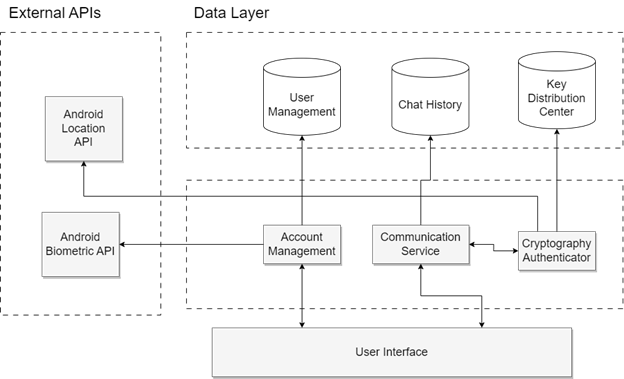
\includegraphics{blockdiagram.png}
% End SubSection

\subsection{Product Functions}
\label{sub:product_functions}
% Begin SubSection
\begin{itemize}
	\item Provide a \emph{summary} of the major functions that the software will perform.
	      \begin{itemize}
		      \item \textbf{Example}: An SRS for an accounting program may use this part to address customer account maintenance, customer statement, and invoice preparation without mentioning the vast amount of detail that each of those functions requires.
	      \end{itemize}
	\item Functions should be organized in a way that makes the list of functions understandable to the customer or to anyone else reading the document for the first time
	\item Present the functions in a list format - each item should be one function, with a brief description of it
	\item Textual or graphical methods can be used to show the different functions and their relationships
	      \begin{itemize}
		      \item Such a diagram is not intended to show a design of a product, but simply shows the logical relationships among variables
	      \end{itemize}
\end{itemize}
% End SubSection

\subsection{User Characteristics}
\label{sub:user_characteristics}
% Begin SubSection
\begin{itemize}
	\item Describe those general characteristics of the intended users of the product including educational level, experience, and technical expertise
	\item Since there will be many users, you may wish to divide into different user types or personas
	      %	\item Do not state specific requirements, but rather provide the reasons why certain specific requirements are later specified
\end{itemize}
% End SubSection

\subsection{Constraints}
\label{sub:constraints}
% Begin SubSection
\begin{itemize}
	\item Provide a general description of any constraints that will limit the developer's options
\end{itemize}
% End SubSection

\subsection{Assumptions and Dependencies}
\label{sub:assumptions_and_dependencies}
% Begin SubSection
\begin{itemize}
	\item List any assumptions you made in interpreting what the software being developed is aiming to achieve
	\item List any other assumptions you made that, if it fails to hold, could require you to change the requirements
	      %\item List each of the factors that affect the requirements stated in the SRS
	      %\item These factors are not design constraints on the software but are, rather, any changes to them that can affect the requirements in the SRS
	      \begin{itemize}
		      \item \textbf{Example}: An assumption may be that a specific operating system will be available on the hardware designated for the software product. If, in fact, the operating system is not available, the SRS would then have to change accordingly.
	      \end{itemize}
\end{itemize}
% End SubSection

\subsection{Apportioning of Requirements}
\label{sub:apportioning_of_requirements}
% Begin SubSection
\begin{itemize}
	\item Identify requirements that may be delayed until future versions of the system
\end{itemize}
% End SubSection

% End Section
\section{Use Case Diagram}
\label{sec:use_case_diagram}
% Begin Section
\begin{itemize}
	\item Provide the use case diagram for the system being developed.
	\item You do not need to provide the textual description of any of the use cases here (these will be specified under "Highlights of Functional Requirements").
	      %	\item Provide \emph{one} use case diagram for the most important Business Event.
	      %	\item The text of all use cases will be specified under "Highlights of Functional Requirements"
\end{itemize}
%In this section, select the most important Business Event that your system responds to and give its use case diagram.  Only one use case diagram is needed.  Give a brief textual description of the use case without repeating what is in the scenarios of the corresponding Business Event.

%
%
%
%This section should provide a use case diagram for your application. 
%\begin{enumerate}[a)]
%	\item Each use case appearing in the diagram should be accompanied by a text description. 
%\end{enumerate}
%% End Section

\section{Highlights of Functional Requirements}
\label{sec:functional_requirements}
% Begin Section
\begin{itemize}
	\item Specify all use cases (or other scenarios triggered by other events), organized by Business Event.
	\item For each Business Event, show the scenario from every Viewpoint. You should have the same set of Viewpoints across all Business Events. If a Viewpoint doesn't participate, write N/A so we know you considered it still. You can choose how to present this - keep in mind it should be easy to follow.
	\item At the end, combine them all into a Global Scenario.
	      %\item Specify the "use cases" (or other triggering events) organized by Business Event. (The Global Scenario is what you might think of as a use case). Be sure to consider Business Events that aren't just triggered by users with goals (e.g. something happens in the environment that your system needs to respond to)
	\item Your focus should be on what the system needs to do, not how to do it. Specify it in enough detail that it clearly specifies what needs to be accomplished, but not so detailed that you start programming or making design decisions.
	\item Keep the length of each use case (Global Scenario) manageable. If it's getting too long, split into sub-cases.
	\item You are \emph{not} specifying a complete and consistent set of functional requirements here. (i.e. you are providing them in the form of use cases/global scenarios, not a refined list). For the purpose of this project, you do not need to reduce them to a list; the global scenarios format is all you need.
	\item Red text below is just to highlight where you need to insert a scenario - don't actually write it all in red.
\end{itemize}

\noindent {\bf Main Business Events:} List out all the main business events you are presenting. If you sub-divided into smaller ones, you don't need to include the smaller ones in this list.\\

\noindent {\bf Viewpoints:} List out all the viewpoints you will be considering.\\

\noindent {\bf Interpretation:} Specify any liberties you took in interpreting business events, if necessary.\\

\begin{enumerate}[{\bf BE1.}]
	\item Business Event Name \#1
	      \begin{enumerate}[{\bf VP1.}]
		      \item Viewpoint Name \#1 \\
		            \textcolor{red}{Insert Scenario Here}
		      \item Viewpoint Name \#2 \\
		            \textcolor{red}{Insert Scenario Here}
	      \end{enumerate}
	      {\bf Global Scenario:}\\
	      \textcolor{red}{Insert Scenario Here}
	\item Business Event Name \#2
	      \begin{enumerate}[{\bf VP1.}]
		      \item Viewpoint Name \#1 \\
		            \textcolor{red}{Insert Scenario Here}
		      \item Viewpoint Name \#2 \\
		            \textcolor{red}{Insert Scenario Here}
	      \end{enumerate}
	      {\bf Global Scenario:}\\
	      \textcolor{red}{Insert Scenario Here}
\end{enumerate}

%	Below, we organize by Business Event.
%	\begin{enumerate}[{BE}1.]
%		\item Business Event name
%		\begin{enumerate}[{VP1}.1]
%			\item Viewpoint name \newline
%			\noindent\fbox{%
%				\parbox{0.5\textwidth}{%
%					\begin{itemize}
%						\item {\bf $S_{1}$:} Initial response of the system to the Business Event
%						\item {\bf $E_{1}$:}  Reaction of the environment to $S_{1}$
%						\item {\bf $S_{2}$:}  Response of the system to $E_{1}$
%						\item {\bf $E_{2}$:}  Reaction of the environment to $S_{2}$
%						\item[] $\cdots$
%						\item {\bf $S_{n}$:}  Response of the system to $E_{(n-1)}$
%						\item {\bf $E_{n}$:}  Reaction of the environment to $E_{(n-1)}$
%						\item {\bf $S_{(n+1)}$:} Final response of the system concluding its function regarding the Business Event
%					\end{itemize}
%				}%
%			}
%			\item Viewpoint name\newline
%			\noindent\fbox{%
%				\parbox{0.5\textwidth}{%
%					\begin{itemize}
%						\item {\bf $S_{1}$:} Initial response of the system to the Business Event
%						\item {\bf $E_{1}$:}  Reaction of the environment to $S_{1}$
%						\item {\bf $S_{2}$:}  Response of the system to $E_{1}$
%						\item {\bf $E_{2}$:}  Reaction of the environment to $S_{2}$
%						\item[] $\cdots$
%						\item {\bf $S_{k}$:}  Response of the system to $E_{(k-1)}$
%						\item {\bf $E_{k}$:}  Reaction of the environment to $E_{(k-1)}$
%						\item {\bf $S_{(k+1)}$:} Final response of the system concluding its function regarding the Business Event
%					\end{itemize}
%				}%
%			}
%			\item \dots
%			\item \dots
%			\item \dots
%			\item[\dots]
%		\end{enumerate}	
%		\item[] {\bf Global Scenario of {\it Business Event Name}:} It is the scenario corresponding to the integration of all the above scenarios from the different Viewpoints of the Business Event BE1.\newline
%		\noindent\fbox{%
%			\parbox{0.5\textwidth}{%
%				\begin{itemize}
%					\item {\bf $S_{1}$:} Initial response of the system to the Business Event
%					\item {\bf $E_{1}$:}  Reaction of the environment to $S_{1}$
%					\item {\bf $S_{2}$:}  Response of the system to $E_{1}$
%					\item {\bf $E_{2}$:}  Reaction of the environment to $S_{2}$
%					\item[] $\cdots$
%					\item {\bf $S_{m}$:}  Response of the system to $E_{(m-1)}$
%					\item {\bf $E_{m}$:}  Reaction of the environment to $E_{(m-1)}$
%					\item {\bf $S_{(m+1)}$:} Final response of the system concluding its function regarding the Business Event
%				\end{itemize}
%			}%
%		}	
%		%\end{enumerate}
%		\item Business Event name
%		\begin{enumerate}[{VP1}.1]
%			\item Viewpoint name \newline
%			\noindent\fbox{%
%				\parbox{0.5\textwidth}{%
%					\begin{itemize}
%						\item {\bf $S_{1}$:} Initial response of the system to the Business Event
%						\item {\bf $E_{1}$:}  Reaction of the environment to $S_{1}$
%						\item {\bf $S_{2}$:}  Response of the system to $E_{1}$
%						\item {\bf $E_{2}$:}  Reaction of the environment to $S_{2}$
%						\item[] $\cdots$
%						\item {\bf $S_{n'}$:}  Response of the system to $E_{(n'-1)}$
%						\item {\bf $E_{n'}$:}  Reaction of the environment to $E_{(n'-1)}$
%						\item {\bf $S_{(n'+1)}$:} Final response of the system concluding its function regarding the Business Event
%					\end{itemize}
%				}%
%			}
%			\item Viewpoint name\newline
%			\noindent\fbox{%
%				\parbox{0.5\textwidth}{%
%					\begin{itemize}
%						\item {\bf $S_{1}$:} Initial response of the system to the Business Event
%						\item {\bf $E_{1}$:}  Reaction of the environment to $S_{1}$
%						\item {\bf $S_{2}$:}  Response of the system to $E_{1}$
%						\item {\bf $E_{2}$:}  Reaction of the environment to $S_{2}$
%						\item[] $\cdots$
%						\item {\bf $S_{k'}$:}  Response of the system to $E_{(k'-1)}$
%						\item {\bf $E_{k'}$:}  Reaction of the environment to $E_{(k'-1)}$
%						\item {\bf $S_{(k'+1)}$:} Final response of the system concluding its function regarding the Business Event
%					\end{itemize}
%				}%
%			}
%			\item \dots
%			\item \dots
%			\item \dots
%			\item[\dots]
%		\end{enumerate}	
%		\item[] {\bf Global Scenario of {\it Business Event Name}:} It is the scenario corresponding to the integration of all the above scenarios from the different Viewpoints of the Business Event BE2.\newline
%		\noindent\fbox{%
%			\parbox{0.5\textwidth}{%
%				\begin{itemize}
%					\item {\bf $S_{1}$:} Initial response of the system to the Business Event
%					\item {\bf $E_{1}$:}  Reaction of the environment to $S_{1}$
%					\item {\bf $S_{2}$:}  Response of the system to $E_{1}$
%					\item {\bf $E_{2}$:}  Reaction of the environment to $S_{2}$
%					\item[] $\cdots$
%					\item {\bf $S_{m'}$:}  Response of the system to $E_{(m'-1)}$
%					\item {\bf $E_{m'}$:}  Reaction of the environment to $E_{(m'-1)}$
%					\item {\bf $S_{(m'+1)}$:} Final response of the system concluding its function regarding the Business Event
%				\end{itemize}
%			}%
%		}		
%	\end{enumerate}

%End Section

\section{Non-Functional Requirements}
\label{sec:non-functional_requirements}


\begin{itemize}
	\item For each non-functional requirement, provide a justification/rationale for it.\\
	      {\bf Example:} \\
	      SC1. \emph{The device should not explode in a customer’s pocket.}\\
	      {\bf Rationale} Other companies have had issues with the batteries they used in their phones randomly exploding [insert citation]. This causes a safety issue, as the phone is often carried in a person's hand or pocket.
	\item If you need to make a guess because you couldn't really talk to stakeholders, you can say "We imagined stakeholders would want...because..."
	\item Each requirement should have a unique label/number for it.
	\item In the list below, if a particular section doesn't apply, just write N/A so we know you considered it.
\end{itemize}

% Begin Section
\subsection{Look and Feel Requirements}
\label{sub:look_and_feel_requirements}
% Begin SubSection

\subsubsection{Appearance Requirements}
\label{ssub:appearance_requirements}
% Begin SubSubSection
\begin{enumerate}[{LF-A}1. ]
	\item
\end{enumerate}
% End SubSubSection

\subsubsection{Style Requirements}
\label{ssub:style_requirements}
% Begin SubSubSection
\begin{enumerate}[{LF-S}1. ]
	\item
\end{enumerate}
% End SubSubSection

% End SubSection

\subsection{Usability and Humanity Requirements}
\label{sub:usability_and_humanity_requirements}
% Begin SubSection

\subsubsection{Ease of Use Requirements}
\label{ssub:ease_of_use_requirements}
% Begin SubSubSection
\begin{enumerate}[{UH-EOU}1. ]
	\item Users should be allowed to report errors and areas of improvement through the organization’s in-app feedback tool. \newline
	      \textbf{Rationale:} The system will provide a way of reporting bugs and errors and provide general feedback or areas of improvement which the organization can then act upon. It will be done through the organization to provide maximum transparency for all stakeholders involved and keep them in the loop about future developments.
	\item On first download, users should be given a short tutorial on the correct usage of the app. \newline
	      \textbf{Rationale:} The tutorial will allow every employee to have a base understanding of the usage of the app and will protect the organization to make sure users properly authenticate before communicating. The tutorial will also indicate certain accessibility features for users that require it to ensure effective usage of the app.
	\item  The system should provide users with a help section including FAQs and recapping the Tutorial. \newline
	      \textbf{Rationale:} While using the app, if a user should face difficulty or forget the location or usage of certain features, they can use the help section to see if their question or problem can be resolved. It will also recap the tutorial including basic usage and accessibility features of the app.
\end{enumerate}
% End SubSubSection

\subsubsection{Personalization and Internationalization Requirements}
\label{ssub:personalization_and_internationalization_requirements}
% Begin SubSubSection
\begin{enumerate}[{UH-PI}1. ]
	\item The system should allow users to change the language to any of the provided languages based on their preferences. \newline
	      \textbf{Rationale:} Users must be able to utilize the app effectively, so it is crucial they understand the different headings and labels within the app. This is also represented within the tutorial as it will be translated into the provided languages. We will only provide languages that the organization uses in day-to-day work as there is an expectation that the employees will understand these languages.
	\item The user should be allowed to change the font based on one’s own preference.  \newline
	      \textbf{Rationale:} Allows the user to customize the font which will apply to all facets of the app for an overall better experience. Some people like different fonts for readability and giving them this option can only raise the overall user experience of using the app.
	\item The user should be allowed to change the background of the chat and home screens. \newline
	      \textbf{Rationale:} Provides users with greater customization to make the app more personal to them. Increasing the options available to the user can improve the user experience and make the app more personal to them.
\end{enumerate}
% End SubSubSection

\subsubsection{Learning Requirements}
\label{ssub:learning_requirements}
% Begin SubSubSection
\begin{enumerate}[{UH-L}1. ]
	\item Users should be able to set up and use the app within 10 minutes of downloading. \newline
	      \textbf{Rationale:} The process for registering a user’s account and then using the app after watching the tutorial should be able to be completed within 10 minutes of the first usage of the app. Keeping the whole set up process short increases user retention using the app and a short, yet comprehensive tutorial ensures that information on usage is more easily understood.
\end{enumerate}
% End SubSubSection

\subsubsection{Understandability and Politeness Requirements}
\label{ssub:understandability_and_politeness_requirements}
% Begin SubSubSection
\begin{enumerate}[{UH-UP}1. ]
	\item Symbols for messaging and adding users should be universally recognized and the standard for all mobile apps. \newline
	      \textbf{Rationale:} To properly utilize the app the user must be able to understand all iconograph. By matching our icons with the ones that are used in other similar apps we can ensure that the average user will be able to seamlessly make the transition to using our app without confusion and contribute to a lower learning curve for the app.
\end{enumerate}
% End SubSubSection

\subsubsection{Accessibility Requirements}
\label{ssub:accessibility_requirements}
% Begin SubSubSection
\begin{enumerate}[{UH-A}1. ]
	\item The user should be allowed to change font size for better visibility.\newline
	      \textbf{Rationale:} This feature should be implemented to ensure ease of use for persons who are more visually impaired. This font size should be global for the app to ensure that users with visual difficulties can always understand what is on the screen.
	\item Implement a colorblind mode which changes the color palette to use more accessible colours. \newline
	      \textbf{Rationale:} This feature should be implemented to ensure ease of use for persons who are colour blind and have difficulty differentiating between colours. The color-blind mode should utilize the Deuteranomaly friendly colour palette so the user can differentiate the colours displayed. [1]
	\item A high contrast/dark color mode should be implemented for better visibility and for usage during nighttime. \newline
	      \textbf{Rationale:} This feature should be implemented to ensure ease of use for people who are more visually impaired and require better distinctions between certain colours. Can be a tool for people who want a dark mode as well and provide better distinction between icons, symbols, and lettering when being used during nighttime or in low lighting. Including a dark mode will greatly increase user experience and provide further customization for the user. [2]

	\item The system should implement an on-screen reader for the visually impaired. \newline
	      \textbf{Rationale:} An on-screen reader is essential for visually impaired people as it allows them to utilize the app more effectively. The on-screen reader should allow for easier navigation through the app as well as provide text-to-speech conversion of messages.

	\item The system should implement a dictation feature which converts voice to messages. \newline
	      \textbf{Rationale:} Provides the user with more methods of performing communication and sending messages. Can help persons with limited dexterity in their fingers by providing an alternative method of communication.

\end{enumerate}
% End SubSubSection

% End SubSection

\subsection{Performance Requirements}
\label{sub:performance_requirements}
% Begin SubSection

\subsubsection{Speed and Latency Requirements}
\label{ssub:speed_and_latency_requirements}
% Begin SubSubSection
\begin{enumerate}[{PR-SL}1. ]
	\item The KDC should have less than a 2-second response time when returning keys. \newline
	      \textbf{Rationale:} The KDC should be able to return keys within 2 seconds of receiving the request from an agent. This time is more than enough to send the key as it does not consider the generation/rotation of keys. This will also ensure agents do not spend a long time waiting to enter a chat due to the KDC having large delays providing a seamless experience.
	\item The time taken to encrypt and decrypt using key should be less than 2s. \newline
	      \textbf{Rationale:} After receiving the key, the encryption and decryption of data should not take longer than 2 seconds since the payload of the data is quite small ranging in the kilobytes of size. We can see that through experimental testing of the algorithms 2 seconds should be more enough to encrypt and decrypt payloads of this size and this represents the worst-case scenario. [3]

	\item The message should be received by the receiving communicating agent in less than  10s after being sent. \newline
	      \textbf{Rationale:} We want to ensure that global standards are met for delivering and receiving messages, but it also needs to be taken into account that these messages are being encrypted and decrypted, which adds extra time. This is why we believe 7.5 seconds is a good realistic timespan in which it doesn’t introduce that large of a delay between send and receive while maintaining a high level of security.

	\item Time taken to access chat logs from the database server should be less than 10 seconds. \newline
	      \textbf{Rationale:} Should an administrator require access to a certain chat log this should be done in a prompt manner and querying data should be fast and efficient. This can aid in Incident Response should there be a security breach, or some other concern related to an employee’s behavior aiding in a fast investigation. 10 seconds provides both a realistic timeframe for querying through large amounts of data while still being prompt in the response time. [4]
\end{enumerate}
% End SubSubSection

\subsubsection{Safety-Critical Requirements}
\label{ssub:safety_critical_requirements}
% Begin SubSubSection
\begin{enumerate}[{PR-SC}1. ]
	\item N/A
\end{enumerate}
% End SubSubSection

\subsubsection{Precision or Accuracy Requirements}
\label{ssub:precision_or_accuracy_requirements}
% Begin SubSubSection
\begin{enumerate}[{PR-PA}1. ]
	\item The app must be only used in accepted locations with an error of location of maximum of 20 meters. \newline
	      \textbf{Rationale:} Most Android Devices utilize some sort of GPS software to ensure accurate location of the device. The average accuracy of GPS enabled devices is around 5m but this can worsen due to location and spotty cell/Wi-Fi service. [5] By expanding the range to 20 meters we account for potential inaccuracies while still maintaining security.

	\item Fingerprint identification should have 99\% accuracy in identifying users. \newline
	      \textbf{Rationale:} The biometric identification feature should have a 99\% accuracy to ensure only authorized users are able to gain entry to the access. This high level of accuracy ensures security by not misidentifying users while still attempting to minimize the total time taken to enter the app by fast identification. It also enables us to use 2-Factor Authentication which is a much more secure method of identification. [6]

\end{enumerate}
% End SubSubSection

\subsubsection{Reliability and Availability Requirements}
\label{ssub:reliability_and_availability_requirements}
% Begin SubSubSection
\begin{enumerate}[{PR-RA}1. ]
	\item The app should have a scheduled downtime of a maximum of 1 hour every 6 months to ensure proper functionality. \newline
	      \textbf{Rationale:} Provides enough time for required maintenance on the app as necessary while maintaining a high level of availability. This higher time of downtime is justified due to the clandestine nature of the app and security being of utmost priority. Since this is a company-wide app it is easy to inform individuals using the app of the scheduled downtime limiting the risk and inconvenience.

	\item The Database server should maintain a backup of the data in cold data storage. \newline
	      \textbf{Rationale:} Ensuring that we keep a backup of the data but stored in cold data storage to save resources as hopefully we will not be needed to access the backup. The accessing of the data in the backup may take a long time if necessary and is primarily used just to ensure data security.

	\item The app should strive for 99.999\% availability during normal operation. \newline
	      \textbf{Rationale:} When the app is being used during standard situations, we should aim for it to have 99.999\% availability as it will ensure that all members of the company remain connected. 99.999\% or 5 nines uptime is industry standard and the highest realistic uptime necessary for the app to maintain continuous availability. [7]


\end{enumerate}
% End SubSubSection

\subsubsection{Robustness or Fault-Tolerance Requirements}
\label{ssub:robustness_or_fault_tolerance_requirements}
% Begin SubSubSection
\begin{enumerate}[{PR-RFT}1. ]
	\item The app should function as long as there is cell service in the area. \newline
	      \textbf{Rationale:} The app should be able to work on mobile data and is not limited to only Wi-Fi. This ensures that communication will still work when Wi-Fi networks are down, ensuring employees can remain connected.

\end{enumerate}
% End SubSubSection

\subsubsection{Capacity Requirements}
\label{ssub:capacity_requirements}
% Begin SubSubSection
\begin{enumerate}[{PR-C}1. ]
	\item The KDC should be able to handle 20\% of the userbase’s requests at the same time. \newline
	      \textbf{Rationale:} Ensures that the KDC meets capacity while also considering scalability in terms of requests. We could say a fixed number such as 20 but if the company has 10000 people with the app there is a high likelihood that more than 20 people request keys at the same time during peak usage of the app. By maintaining this requirement as a percentage, we can maintain both scalability and have good capacity throughput.
	\item The Initial Database Server should have a minimum of 1TB storage before scaling. \newline
	      \textbf{Rationale:}  We want to have a large base server size to ensure that we do not need to start scaling unnecessarily expending valuable resources on maintaining the database. 1TB of storage can store multiple years worth of data without

\end{enumerate}
% End SubSubSection

\subsubsection{Scalability or Extensibility Requirements}
\label{ssub:scalability_or_extensibility_requirements}
% Begin SubSubSection
\begin{enumerate}[{PR-SE}1. ]
	\item The app should maintain at least 5\% of the database empty to ensure space for future chat logs. \newline
	      \textbf{Rationale:} Allow for scalability to store more chat logs in the future. Ensure that we never reach a situation where there are chats coming in but not being stored due to the full capacity in the database server. 5\% also provides a good buffer space if there is a sudden influx of data providing time for the database to scale to the new capacity.

\end{enumerate}
% End SubSubSection

\subsubsection{Longevity Requirements}
\label{ssub:longevity_requirements}
% Begin SubSubSection
\begin{enumerate}[{PR-L}1. ]
	\item The app in its first iteration must be able to last a minimum of 2 years with avenues for extension or improvement. \newline
	      \textbf{Rationale:} Current iteration should be usable by employees and based on feedback and bug reporting we can provide future updates or overhauls. This process could take a long time so it is important the current iteration lasts at least 2 years for feedback to be collected and updates developed.

\end{enumerate}
% End SubSubSection

% End SubSection

\subsection{Operational and Environmental Requirements}
\label{sub:operational_and_environmental_requirements}
% Begin SubSection

\subsubsection{Expected Physical Environment}
\label{ssub:expected_physical_environment}
% Begin SubSubSection
\begin{enumerate}[{OE-EPE}1. ]
	\item
\end{enumerate}
% End SubSubSection

\subsubsection{Requirements for Interfacing with Adjacent Systems}
\label{ssub:requirements_for_interfacing_with_adjacent_systems}
% Begin SubSubSection
\begin{enumerate}[{OE-IA}1. ]
	\item
\end{enumerate}
% End SubSubSection

\subsubsection{Productization Requirements}
\label{ssub:productization_requirements}
% Begin SubSubSection
\begin{enumerate}[{OE-P}1. ]
	\item
\end{enumerate}
% End SubSubSection

\subsubsection{Release Requirements}
\label{ssub:release_requirements}
% Begin SubSubSection
\begin{enumerate}[{OE-R}1. ]
	\item
\end{enumerate}
% End SubSubSection

% End SubSection

\subsection{Maintainability and Support Requirements}
\label{sub:maintainability_and_support_requirements}
% Begin SubSection

\subsubsection{Maintenance Requirements}
\label{ssub:maintenance_requirements}
% Begin SubSubSection
\begin{enumerate}[{MS-M}1. ]
	\item
\end{enumerate}
% End SubSubSection

\subsubsection{Supportability Requirements}
\label{ssub:supportability_requirements}
% Begin SubSubSection
\begin{enumerate}[{MS-S}1. ]
	\item
\end{enumerate}
% End SubSubSection

\subsubsection{Adaptability Requirements}
\label{ssub:adaptability_requirements}
% Begin SubSubSection
\begin{enumerate}[{MS-A}1. ]
	\item
\end{enumerate}
% End SubSubSection

% End SubSection

\subsection{Security Requirements}
\label{sub:security_requirements}
% Begin SubSection

\subsubsection{Access Requirements}
\label{ssub:access_requirements}
% Begin SubSubSection
\begin{enumerate}[{SR-AC}1. ]
	\item
\end{enumerate}
% End SubSubSection

\subsubsection{Integrity Requirements}
\label{ssub:integrity_requirements}
% Begin SubSubSection
\begin{enumerate}[{SR-INT}1. ]
	\item
\end{enumerate}
% End SubSubSection

\subsubsection{Privacy Requirements}
\label{ssub:privacy_requirements}
% Begin SubSubSection
\begin{enumerate}[{SR-P}1. ]
	\item
\end{enumerate}
% End SubSubSection

\subsubsection{Audit Requirements}
\label{ssub:audit_requirements}
% Begin SubSubSection
\begin{enumerate}[{SR-AU}1. ]
	\item
\end{enumerate}
% End SubSubSection

\subsubsection{Immunity Requirements}
\label{ssub:immunity_requirements}
% Begin SubSubSection
\begin{enumerate}[{SR-IM}1. ]
	\item
\end{enumerate}
% End SubSubSection

% End SubSection

\subsection{Cultural and Political Requirements}
\label{sub:cultural_and_political_requirements}
% Begin SubSection

\subsubsection{Cultural Requirements}
\label{ssub:cultural_requirements}
% Begin SubSubSection
\begin{enumerate}[{CP-C}1. ]
	\item
\end{enumerate}
% End SubSubSection

\subsubsection{Political Requirements}
\label{ssub:political_requirements}
% Begin SubSubSection
\begin{enumerate}[{CP-P}1. ]
	\item
\end{enumerate}
% End SubSubSection

% End SubSection

\subsection{Legal Requirements}
\label{sub:legal_requirements}
% Begin SubSection

\subsubsection{Compliance Requirements}
\label{ssub:compliance_requirements}
% Begin SubSubSection
\begin{enumerate}[{LR-COMP}1. ]
	\item
\end{enumerate}
% End SubSubSection

\subsubsection{Standards Requirements}
\label{ssub:standards_requirements}
% Begin SubSubSection
\begin{enumerate}[{LR-STD}1. ]
	\item
\end{enumerate}
% End SubSubSection

% End SubSection

% End Section

\appendix
\section{Division of Labour}
\label{sec:division_of_labour}
% Begin Section
Include a Division of Labour sheet which indicates the contributions of each team member. This sheet must be signed by all team members.
\subsection*{Virochaan Ravichandran Gowri:}
\begin{itemize}
	\item 1.1 - Purpose
	\item 2.1 - Product Perspective
	\item 2.1 - Block Diagram showcasing product connections
	\item 5.2, 5.3 - Usability and Humanity + Performance Non Functional Requirements.
	\item Reviewed the whole document as a group
\end{itemize}

% End Section

%\newpage
%\section*{IMPORTANT NOTES}
%\begin{itemize}
%	\item Be sure to include all sections of the template in your document regardless whether you have something to write for each or not
%	\begin{itemize}
%		\item If you do not have anything to write in a section, indicate this by the \emph{N/A}, \emph{void}, \emph{none}, etc.
%	\end{itemize}
%	\item Uniquely number each of your requirements for easy identification and cross-referencing
%	\item Highlight terms that are defined in Section~1.3 (\textbf{Definitions, Acronyms, and Abbreviations}) with \textbf{bold}, \emph{italic} or \underline{underline}
%	\item For Deliverable 1, please highlight, in some fashion, all (you may have more than one) creative and innovative features. Your creative and innovative features will generally be described in Section~2.2 (\textbf{Product Functions}), but it will depend on the type of creative or innovative features you are including.
%\end{itemize}


\end{document}
%------------------------------------------------------------------------------